\documentclass[../main/thesis.tex]{subfiles}
\begin{document}
\newpage
%% Electronics

\chapter{Choice of Readout Electronics for the 3DMiMic Detector}
\label{e}

\section{Detector Readout}
\label{t-read}
In different situations, the desired output from the detector readout will be different. In some cases, it is enough to simply count the radiation quanta, and in other cases one might want to read out a energy spectrum. In both cases the readout chain starts with a pre-amplifier that produces a voltage that is proportional to the radiation charge. The output from the pre-amplifier is sent to a shaping amplifier which converts the signal to a shape that is more suitable for the next component in the readout chain. This is to select the interesting pulses and convert the analog signal to a digital signal in one way or another. \citep[chap. 16]{Knoll}

\subsection{Pre-Amplifier}
\label{t-amp}
For most radiation detectors, the liberated charge is too small to be processed, which is why pre-amplifiers are needed in most detector readout chains. The pre-amplifier is located close to the detector to reduce noise. A pre-amplifier can be voltage-sensitive or charge-sensitive. A voltage-sensitive pre-amplifier has an output signal proportional to the input voltage, which will be proportional to the input charge if the detector capacitance is constant. This is not the case for semiconductor detectors where the capacitance may change with the operating parameters. A \gls{CSA} has a output signal that is independent of the input capacitance as long as the amplifier gain is high enough compared to a relationship between capacitances in the system. \citep[chap. 16]{Knoll}
%fig 16.13?

One often important parameter to consider in a pre-amplifier is the dynamic range, which is the range of input signal amplitudes that can be reliably measured without changing the system. The lowest measurable input signal is limited by the noise in the system, mainly in the detector, detector cables, and pre-amplifier. A signal is not reliable if it is difficult to discern from the noise. The highest measurable input signal can be limited by the pre-amplifier or later stages, like the \gls{ADC}. If the pre-amplifier has a high gain, then a large input signal will require a higher output signal than the pre-amplifier can deliver. If the gain is low, then another stage in the system will likely be the bottleneck before the pre-amplifier reaches its highest output level. \citep{dynamic-range}

It is typically convenient to use the pre-amplifier to supply bias voltage to the detector. When this is done a single cable is used both to provide voltage to the detector and to transfer the signal pulses to the readout system. \citep[chap. 16]{Knoll}
%fig 16.16a?

\subsubsection{Charge-Sensitive Amplifier Operation}
\label{t-csa}
\begin{figure}%[h]
	\centering
	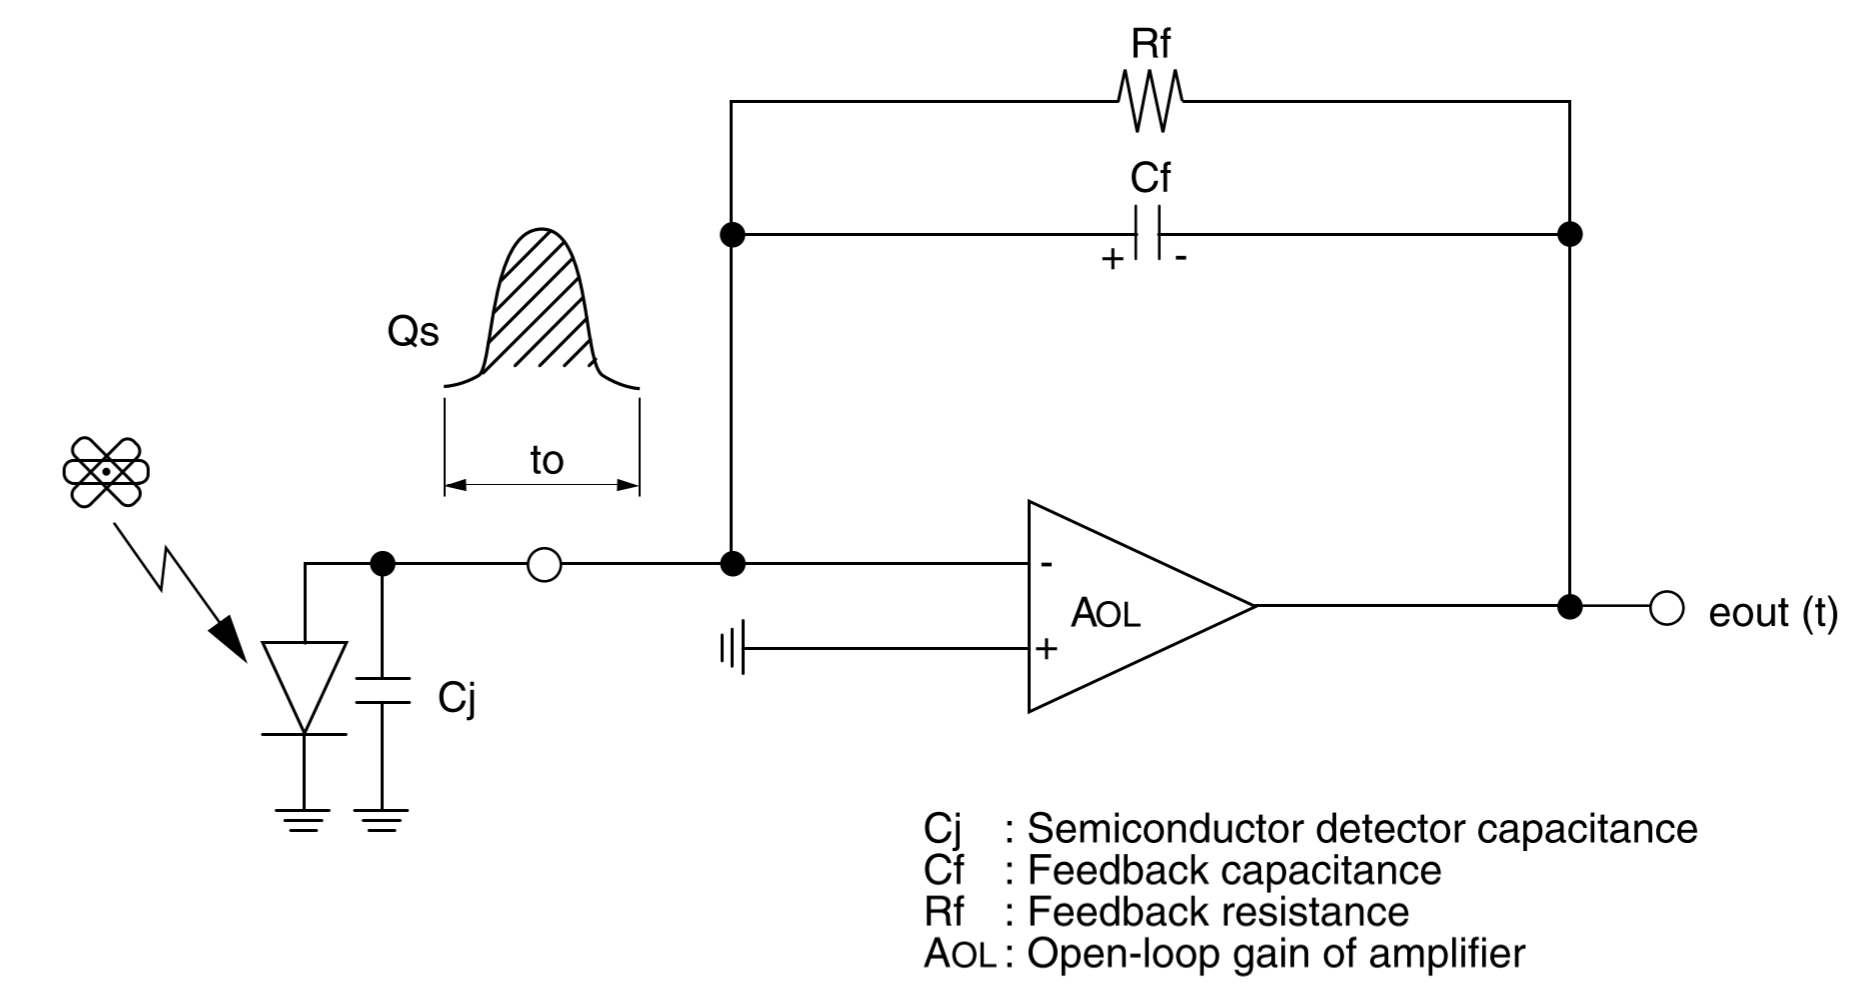
\includegraphics[width=\textwidth]{csa.png}
	\caption{Schematic of a basic \gls{CSA}. \citep{Hamamatsu}}
	\label{fig-csa}
\end{figure}

Figure \ref{fig-csa} shows a general \gls{CSA}. When a radiation quanta strikes the detector, a pulse of charge $Q_s$ and width $t_o$ is generated. This creates a rising potential on the negative input of the amplifier, which triggers a falling potential on the output of the amplifier. Because of the negative feedback, this will quickly draw the negative input close to zero, making the negative input a point of virtual ground. The feedback currents charge the feedback capacitor, and then the capacitor is slowly discharged when there is no signal on the input. This creates a voltage pulse on the output that slowly falls from a peak value that is proportional to the input charge. \citep{Hamamatsu}

\subsection{Shaper}
\label{t-shaper}
The shaper, or shaping amplifier, converts the shape of the signal to a form that is suitable for measurement. The pulse height of the signal from the shaper is proportional to the input charge. It is important that the output from the shaper quickly returns to the baseline to prevent pulse overlapping that will cause measurement errors. The first stage of the shaper is a differentiator (high pass filter) which passes the steep rise of the input pulse, but quickly returns to the baseline. The differentiator decides the fall time of the pulse. The signal is then amplified to a level that is suitable for the \gls{ADC}, before it is passed through the integrator (low pass filter) that filters away noise and changes the rise time of the pulse. The duration of the shaped pulse is called the shaping time. \citep[chap. 16]{Knoll}

%discriminator?

\subsection{Analog-to-Digital Conversion}
\label{t-adc}
The analog signal from the shaper needs to be converted to a digital signal for processing and storage. When it is desired to keep as much information as possible, an \gls{ADC} is used, but these use a lot of area and power. In situations where area, power, and cost is more important than accuracy of measurements (typically when there are a lot of channels), there are some simpler methods that can be used instead. The simplest is a counter, which merely counts the number of pulses with a height above a defined threshold. The information on the radiation quanta energy is lost, but the circuit is very simple. It is also possible to have multiple counters with different thresholds, which will keep some information about the distribution of radiation quanta energies. Another much used method is the \gls{ToT} technique. A \gls{ToT} circuit measures the time that the pulse is over a defined threshold, and then this measurement can be used to estimate the height of the pulse. The relationship between pulse height and \gls{ToT} is only linear within a certain range, and will usually limit the dynamic range of the readout system. \citep[chap. 6]{ToT}

%This link for ADC vs ToT: https://books.google.no/books?id=DFDRBQAAQBAJ&pg=PA173&lpg=PA173&dq=time+over+threshold+energy+measurement&source=bl&ots=J7wJ9nACVW&sig=ra60jHHnJxCc7g3g1TV2RLwHjqU&hl=en&sa=X&ved=0CBsQ6AEwADgKahUKEwi-zcfjuZTJAhUKnnIKHSQ4BAI#v=onepage&q=time%20over%20threshold%20energy%20measurement&f=false

An \gls{ADC} samples the analog signal amplitude at a certain interval (sampling rate) and converts each sampled value to a digital signal. The resolution, which is the number of bits in the digital signal, will limit the accuracy of the conversion. The quantisation error is introduced as each analog value needs to be converted to the closest digital value. The maximum percentage quantisation error can be seen in equation \ref{eq-eqmax}, where n is the number of digits in the binary code and $2^n$ is the number of digital values. \citep[chap. 10]{Bentley}

\begin{equation}%[h]
e_q^{MAX} = \pm \frac{100}{2(2^n - 1)}\%
\label{eq-eqmax}
\end{equation}

The dynamic range of an \gls{ADC} will mainly be limited by its resolution, noise, linearity, and jitter (small timing errors). %https://en.wikipedia.org/wiki/Analog-to-digital_converter
%Types of ADC?

\subsection{Digital Signal Processing}
\label{t-dsp}

%\subsection{Medipix}
%\label{t-medipix}

\section{Medipix and Timepix}
\label{e-medipix}
Medipix is a family of chips developed to exploit technology from the experiments at CERN in other fields of science, mainly medical imaging. The chips made by the Medipix collaboration are; Medipix1, Medipix2, Timepix, Medipix3, Timepix3, and Dosepix. The Medipix 1-3 chips are made for photon counting and are therefore not useful for dosimetry. The Timepix chips are made to do \gls{ToT} measurements, with Timepix and Timepix3 being based on Medipix2 and Medipix3 respectively. Dosepix is a currently in development chip made for photon dosimetry. Timepix3 and Dosepix were considered for the 3DMiMic project, but as \gls{ToT} devices their dynamic range is not very large. Also, since they are made for photon detectors they cannot read the large charges released by a carbon ion in the Bragg peak. 

\section{UiO Portable Front-End Readout System}
\label{e-uio}
During the school year 2014-2015 two master students at \gls{uio} made a portable front-end readout system for radiation detectors \citep{tali} \citep{oltedal}. This system consists of two custom made cards and a \gls{FPGA} evaluation board. The first card, the analog card, has three channels with pre-amplifiers while two of those channels also including shapers. The second card, the digital card, includes an \gls{ADC}, comparators, and current monitors. The components of the digital card is connected to the \gls{FPGA} on the SoCKit evaluation board by Arrow, which is connected to a computer through network. The system is made to detect fission fragments which produce very large signals, and therefore has a low gain. This makes the system too noisy for the low noise requirements of the 3DMiMic detector at the default gain, but this can be changed using external components.

\section{IDEAS Amadeus Preamp-Shaper}
\label{e-ide1180}
IDE1180, or Amadeus, by Oslo-based IDEAS is an integrated circuit for the front-end readout of radiation detectors. It features 16 channels of \gls{CSA} and shapers with adjustable shaping time. The preliminary datasheet \citep{IDE1180} specifies a shaping time between 20~ns and 40~ns, negative and positive input charges up to 400~fC with lowest gain, and equivalent noise charge of 1106~e- plus 68~e- per pF load at default gain. 

This chip was considered by multiple projects at \gls{ift} and a evaluation board (7045) was given to \gls{ift} so that more extensive tests could be performed. 

\section{Ortec 142A Pre-Amplifier}
\label{e-ortec}
Ortec 142A is a single channel low-noise \gls{CSA} optimized for charged particle or heavy-ion detectors. It was considered for the 3DMiMic project since \gls{uib} already owns a few of these. It features a very high dynamic range, but the gain is too low for the 3DMiMic detector. 

\section{Portable PCIe ADC System}
\label{e-adc}
The current \gls{ADC} system used at \gls{uib} is a Caen V1729A digitizer sitting in a VMI crate. This features four 14 bit channels with 2~GS/s sampling rate, but is very large and heavy, making it cumbersome to bring for radiation tests. It was desirable to purchase a new \gls{ADC} for the department that could be put inside a small computer using PCI Express (PCIe) to make a portable system. Three manufacturers that produced suitable \gls{ADC}s for a reasonable price were found; AlazarTech, Keysight Technologies, and SP Devices. The considered models are listed in table~\ref{tab-adc}. 

\begin{table}[h]
\begin{center}
	\caption{The analog-to-digital converters considered for purchase.}
	\label{tab-adc}
	\begin{tabular}{| c | c | c | c | c |}
		\hline
		Manufacturer & Model & Channels & Resolution & Sampling \\ 
		 & & & (bits) & (GS/s) \\ \hline
		AlazarTech & ATS9360 & 2 & 12 & 1.8 \\ \hline
		Keysight & U5303A & 2 (1) & 12 & 1.6 (3.2) \\ \hline
		SP Devices & ADQ14AC-2X & 2 & 14 & 2 \\ \hline
		SP Devices & ADQ14AC-4C & 4 & 14 & 1 \\ \hline
	\end{tabular}
\end{center}
\end{table}

The Keysight model was interesting with a signal interleaving feature where both 1.6~GS/s channels could be combined into one 3.2~GS/s channel. In the end SP Devices was chosen, being the only discovered company that produces 14 bit PCIe \gls{ADC}s in the GS/s range. ADQ14AC-4C was chosen as having two extra channels was considered more important than higher sampling rate for radiation tests. The old Caen \gls{ADC} can be used for projects and tests that require higher sampling rate. 



\end{document}